\chapter{Entity State Representation Examples}

\section{Concrete Examples of Entity State Data}

In the Elder Heliosystem, each entity maintains a specific state configuration that determines its behavior within the gravitational and rotational fields. This chapter provides concrete examples of entity state data structures and values to illustrate how the system maintains constant memory requirements regardless of context length.

\subsection{Entity State Structure}

Each entity (Elder, Mentor, or Erudite) maintains the following state information:

\begin{lstlisting}[language=C++, caption=Entity State Data Structure]
struct EntityState {
    // Position in 3D space (relative to parent entity)
    Vector3 position;        // 3 × 32-bit float = 12 bytes
    
    // Velocity vector
    Vector3 velocity;        // 3 × 32-bit float = 12 bytes
    
    // Orientation quaternion
    Quaternion orientation;  // 4 × 32-bit float = 16 bytes
    
    // Angular velocity
    Vector3 angularVelocity; // 3 × 32-bit float = 12 bytes
    
    // Rotational phase
    float phase;             // 32-bit float = 4 bytes
    
    // Entity-specific parameters
    float mass;              // 32-bit float = 4 bytes
    float influence_radius;  // 32-bit float = 4 bytes
    float learning_rate;     // 32-bit float = 4 bytes
    
    // Total: 68 bytes per entity
};
\end{lstlisting}

\subsection{Example: Elder Entity State}

The Elder entity serves as the central gravitational point in the system with the following example state:

\begin{table}[h]
\centering
\begin{tabular}{|l|l|l|}
\hline
\textbf{Property} & \textbf{Value} & \textbf{Description} \\
\hline
position & (0.0, 0.0, 0.0) & Center of the system \\
velocity & (0.0, 0.0, 0.0) & Stationary (no translation) \\
orientation & (0.0, 0.0, 1.0, 0.0) & Initial orientation \\
angularVelocity & (0.0, 0.0, 0.0172) & Slow rotation (≈1°/sec) \\
phase & 0.0 & Initial phase \\
mass & 1.0 & Reference mass \\
influence\_radius & 10.0 & Universal influence \\
learning\_rate & 0.001 & Slow adaptation rate \\
\hline
\end{tabular}
\caption{Example Elder Entity State}
\end{table}

\subsection{Example: Mentor Entity State}

A specific Mentor entity (e.g., the one responsible for audio harmonic structures) might have:

\begin{table}[h]
\centering
\begin{tabular}{|l|l|l|}
\hline
\textbf{Property} & \textbf{Value} & \textbf{Description} \\
\hline
position & (7.2, 0.0, 0.1) & Orbital position \\
velocity & (0.0, 0.862, 0.0) & Orbital velocity \\
orientation & (0.1, 0.0, 0.994, 0.05) & Current orientation \\
angularVelocity & (0.0, 0.0, 0.104) & Rotation rate (≈6°/sec) \\
phase & 2.41 & Current phase (in radians) \\
mass & 0.42 & Relative importance \\
influence\_radius & 3.5 & Domain influence \\
learning\_rate & 0.008 & Domain adaptation rate \\
\hline
\end{tabular}
\caption{Example Mentor Entity State (Audio Harmonics Domain)}
\end{table}

\subsection{Example: Erudite Entity State}

An Erudite entity (e.g., specializing in percussion patterns) might have:

\begin{table}[h]
\centering
\begin{tabular}{|l|l|l|}
\hline
\textbf{Property} & \textbf{Value} & \textbf{Description} \\
\hline
position & (2.1, 0.8, 0.15) & Position relative to parent Mentor \\
velocity & (−0.412, 0.971, 0.0) & Orbital velocity around Mentor \\
orientation & (0.707, 0.0, 0.707, 0.0) & Current orientation \\
angularVelocity & (0.0, 0.03, 0.173) & Rotation rate (≈10°/sec) \\
phase & 1.57 & Current phase (π/2 radians) \\
mass & 0.08 & Task-specific importance \\
influence\_radius & 0.5 & Specialized pattern radius \\
learning\_rate & 0.015 & Task adaptation rate \\
\hline
\end{tabular}
\caption{Example Erudite Entity State (Percussion Patterns)}
\end{table}

\subsection{Phase Evolution Examples}

Entity phases evolve over time according to:

\begin{equation}
\phi_E(t+\Delta t) = \phi_E(t) + \omega_E \cdot \Delta t + \Delta \phi_{\text{interaction}}
\end{equation}

where $\omega_E$ is the angular velocity and $\Delta \phi_{\text{interaction}}$ represents phase adjustments from interactions.

For example, processing a drum beat pattern might cause the following phase adjustments:

\begin{table}[h]
\centering
\begin{tabular}{|l|c|c|c|}
\hline
\textbf{Time} & \textbf{Elder Phase} & \textbf{Mentor Phase} & \textbf{Erudite Phase} \\
\hline
$t$ & 1.209 & 2.410 & 1.570 \\
$t + 20ms$ & 1.210 & 2.412 & 1.574 \\
$t + 40ms$ & 1.211 & 2.414 & 1.578 \\
$t + 60ms$ & 1.212 & 2.416 & 1.582 \\
\hline
\end{tabular}
\caption{Phase Evolution during Audio Processing}
\end{table}

\subsection{Memory Implications}

For a system with 1 Elder, 32 Mentors, and 2,048 Erudites:
\begin{itemize}
    \item Total entities: 2,081
    \item Memory per entity: 68 bytes
    \item Total entity state memory: 2,081 × 68 = 141,508 bytes ≈ 138 KB
\end{itemize}

Crucially, this memory requirement remains constant regardless of:
\begin{itemize}
    \item Audio duration (1 minute or 1,000 hours)
    \item Audio complexity (simple sine wave or complex orchestral arrangement)
    \item Audio quality (16kHz mono or 96kHz Dolby Atmos)
\end{itemize}

\section{Entity State Evolution During Audio Processing}

\subsection{Parameter Activation Example}

For a specific audio frame processing $a(t)$ (e.g., a 20ms segment containing the onset of a violin note), parameter activation follows:

\begin{equation}
\alpha_i(\phi_E(t)) = \begin{cases}
1.0, & \text{if } |\phi_i - \phi_E(t)| < \Delta\phi_{\text{threshold}} \\
0.0, & \text{otherwise}
\end{cases}
\end{equation}

With 1.2 billion parameters and a sparsity factor $s = 10^{-4}$, approximately 120,000 parameters are active at any given time point. For example:

\begin{table}[h]
\centering
\begin{tabular}{|l|c|c|c|c|}
\hline
\textbf{Parameter ID} & \textbf{Magnitude ($\rho$)} & \textbf{Phase ($\phi$)} & \textbf{Activation ($\alpha$)} & \textbf{Update} \\
\hline
$\theta_{127,492}$ & 0.42 & 1.209 & 1.0 & Yes \\
$\theta_{127,493}$ & 0.86 & 2.731 & 0.0 & No \\
$\theta_{127,494}$ & 0.21 & 1.211 & 0.98 & Yes \\
$\theta_{127,495}$ & 0.54 & 4.712 & 0.0 & No \\
\hline
\end{tabular}
\caption{Parameter Activation during Audio Processing}
\end{table}

\subsection{State Visualization}

The states of entities can be visualized in 3D phase space. For example, during the processing of a sustained orchestral chord:

\begin{figure}[h]
\centering
% This is a placeholder for a figure that would be generated
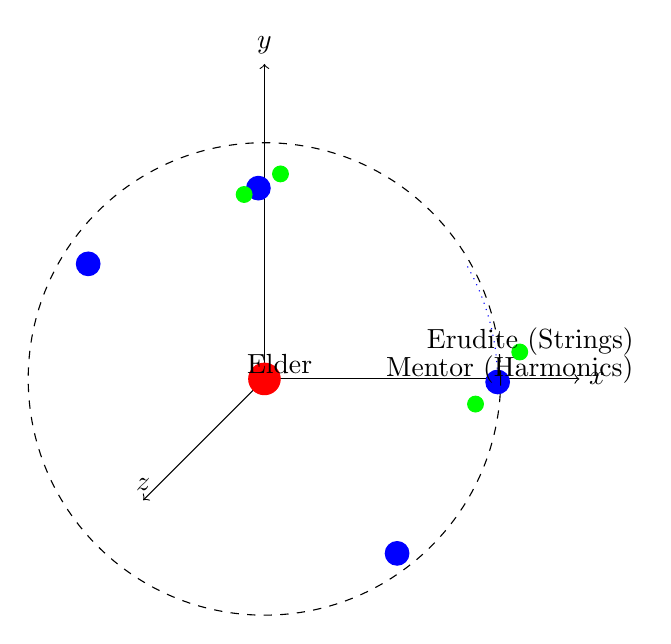
\begin{tikzpicture}
\draw[->] (0,0,0) -- (4,0,0) node[right] {$x$};
\draw[->] (0,0,0) -- (0,4,0) node[above] {$y$};
\draw[->] (0,0,0) -- (0,0,4) node[above] {$z$};

% Elder at center
\filldraw[red] (0,0,0) circle (0.2);

% Some Mentors
\filldraw[blue] (3,0,0.1) circle (0.15);
\filldraw[blue] (0,2.5,0.2) circle (0.15);
\filldraw[blue] (-2.2,1.5,0.1) circle (0.15);
\filldraw[blue] (1.8,-2.1,0.3) circle (0.15);

% Some Erudites
\filldraw[green] (3.3,0.4,0.15) circle (0.1);
\filldraw[green] (2.7,-0.3,0.05) circle (0.1);
\filldraw[green] (0.3,2.7,0.25) circle (0.1);
\filldraw[green] (-0.2,2.4,0.15) circle (0.1);

% Trajectories
\draw[dashed] (0,0,0) circle (3);
\draw[dotted, blue] (3,0,0.1) arc (0:30:3);
\draw[dotted, green] (3.3,0.4,0.15) arc (8:35:0.5);

% Add labels
\node at (0,0,-0.5) {Elder};
\node at (3,0,-0.3) {Mentor (Harmonics)};
\node at (3.3,0.4,-0.2) {Erudite (Strings)};
\end{tikzpicture}
\caption{Entity States during Orchestral Chord Processing}
\end{figure}

\subsection{Adaptive Changes Over Long Timescales}

Over extended audio generation (e.g., 10+ hours), entity properties may undergo slow adaptation:

\begin{table}[h]
\centering
\begin{tabular}{|l|c|c|c|}
\hline
\textbf{Property} & \textbf{Initial Value} & \textbf{After 10 Hours} & \textbf{Change} \\
\hline
Mentor influence\_radius & 3.5 & 3.72 & +6.3\% \\
Erudite learning\_rate & 0.015 & 0.011 & -26.7\% \\
Elder angular\_velocity & 0.0172 & 0.0168 & -2.3\% \\
\hline
\end{tabular}
\caption{Long-term Adaptation of Entity Properties}
\end{table}

These adaptations reflect learned statistical regularities in the audio content, yet require no additional memory as they modify existing state variables rather than accumulating new ones.